\subsection{Computing Architectures}

\subsubsection{Cloud Computing}

\definition{Cloud Computing} is a coherent, large-scale, publicly accessible \textbf{collection of computing, storage and networking resources}. It is usually available via web service calls over the Internet. The business is based on short or long term access on a pay-per-use basis.

\highspace
The \textbf{cloud is implemented through virtualization}. This involves \textbf{partitioning hardware resources} (CPU, RAM, etc.) \textbf{and sharing them between multiple virtual machines} (VMs). This model ensures performance isolation and security. The Virtual Machine Monitor (VMM) manages access to physical resources between running VMs. The pros and cons of virtualization are explained in the dedicated chapter \ref{subsection: virtualization} (page \pageref{subsection: virtualization}).

\longline

\paragraph{Server Consolidation}

\definition{Server Consolidation} in cloud computing refers to the \textbf{process of combining multiple servers into a single, more powerful server or cluster of servers}.

\highspace
This can be done to \textbf{improve the efficiency and cost effectiveness of the cloud computing environment}.

\highspace
Server Consolidation is typically \textbf{achieved through the use of virtualization technology}, which allows \textbf{multiple virtual servers to run on a single physical server}. This enables better utilization of resources, as well as improved scalability and flexibility. It also allows organizations to reduce the number of physical servers they need to maintain, which can lead to cost savings on hardware, power and cooling. 

\highspace
In the context of server consolidation, \definition{Consolidation Management} is the \textbf{migration from physical to virtual machines}.

\highspace
Let us just say that the \textbf{characteristics} of this technique are:
\begin{itemize}
	\item \textbf{\underline{Scalability}}. It is possible to \textbf{move VMs without disrupting the applications running in them}.
	
	\item \textbf{\underline{Automatic scalability}}. In addition to scalability, it is also possible to \textbf{automatically balance workloads according to set limits and guarantees}.
	
	\item \textbf{\underline{High availability}}. Servers and applications are \textbf{protected against component and system failures}.
\end{itemize}
\newpage
\begin{flushleft}
	\textcolor{Green3}{\faIcon{question-circle} \textbf{Server Consolidation Advantages}}
\end{flushleft}
The benefits of server consolidation are:
\begin{itemize}
	\item \textbf{Different operating systems can run on the same hardware}.
	
	\item Higher hardware utilization means \textbf{less hardware is needed} (\textbf{lower acquisition} and \textbf{maintenance costs}).
	
	\item Continued use of legacy software.
	
	\item \textbf{Application independent of hardware}.
\end{itemize}

\longline

\paragraph{Services provided by cloud}

\definition{Cloud Computing} is a \textbf{model for} providing convenient, \textbf{on-demand network access to a shared pool of configurable computing resources}, such as networks, servers, storage, applications and services. Anything that can be \textbf{quickly provisioned and released with minimal management} or interaction with the service provider.

\highspace
\dquotes{\definition{X as a service}} (rendered as \texttt{*aaS} in acronyms) is a phrasal template for any business model in which a product use is offered as a subscription-based service rather than as an artifact owned and maintained by the customer.\cite{bhattacharya2022xaas} 

There is a wide variety of \dquotes{\definition{as-a-Service}} terms used to describe services offered in clouds.

\begin{multicols}{2}
	\begin{itemize}
		\item AaaS - Architecture as a Service
		\item BaaS - Business as a Service
		\item CaaS - Communication as a Service
		\item CRMaaS - CRM as a Service
		\item DaaS - Data as a Service
		\item DBaaS - Database as a Service
		\item EaaS - Ethernet as a Service
		\item FaaS - Frameworks/Function as a Service
		\item GaaS - Globalization/Governance as a Service
		\item HaaS - Hardware as a Service
		\item IaaS - Infrastructure/Integration as a Service
		\item IDaaS - Identity as a Service
		\item ITaaS - IT as a Service
		\item LaaS - Lending as a Service
		\item MaaS - Mashups as a Service
		\item OaaS - Organization/Operations as a Service
		\item SaaS - Software as a Service
		\item StaaS - Storage as a Service
		\item PaaS - Platform as a Service
		\item TaaS - Technology/Testing as a Service
		\item VaaS - Voice as a Service
	\end{itemize}
\end{multicols}

\newpage

\noindent
The \textbf{main services} provided by the cloud are shown in the image below.

\begin{figure}[!htp]
	\centering
	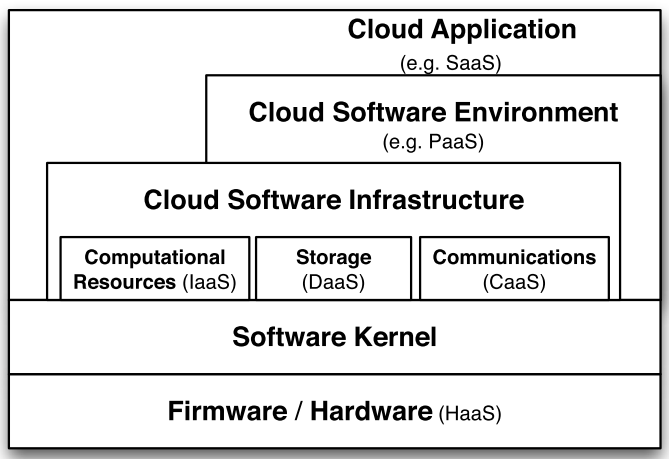
\includegraphics[width=.8\textwidth]{img/as-a-service-1.png}
\end{figure}

\begin{itemize}
	\item \definition{Cloud Application Layer}: SaaS (Software as a Service). \textbf{Users access the services provided by this layer through web portals and may be charged for using them}.
	
	Cloud applications can be developed on the cloud software environments or infrastructure components. 
	
	Some \example{examples} include \href{https://www.google.com/intl/en/gmail/about/}{Gmail}, \href{https://www.webex.com/}{Webex}, \href{https://www.google.com/intl/en/docs/about/}{Google Docs}.
	
	
	\item \definition{Cloud Software Environment Layer}: PaaS (Platform as a Service). Users are \textbf{application developers}.
	
	\textbf{Vendors provide} developers with a \textbf{programming language level environment with a well-defined API}. It has many advantages:
	\begin{itemize}
		\item Ease the interaction between the environment and applications.
		\item Accelerate deployment.
		\item Support scalability.
	\end{itemize}
	
	Some \example{examples} are \href{https://aws.amazon.com/lambda/}{Amazon Lambda} and \href{https://azure.microsoft.com/en-US}{Microsoft Azure}.
	
	
	\item \definition{Cloud Software Infrastructure Layer}: provides resources to the higher-level layers.
	\begin{itemize}
		\item \textbf{Computational Resources Layer}: IaaS (Infrastructure as a Service). The vendor provides \textbf{virtual machines to developers}. Then the pros and cons are related to the virtual machines.
		
		\begin{flushleft}
			\textcolor{Green3}{\faIcon{check-circle} \textbf{Advantages}}
		\end{flushleft}
		\begin{itemize}
			\item Flexibility.
			\item Root access to the virtual machine to fine-tune settings and customize installed software.
		\end{itemize}
		\newpage
		\begin{flushleft}
			\textcolor{Red2}{\faIcon{thumbs-down} \textbf{Disadvantages}}
		\end{flushleft}
		\begin{itemize}
			\item Performance impact.
			\item Inability to provide strong SLA guarantees.
		\end{itemize}
		Some examples are \href{https://aws.amazon.com/ec2/}{Amazon EC2}, \href{https://cloud.google.com/products/compute?hl=en}{Google Compute Engine}, \href{https://www.ibm.com/cloud}{IBM Cloud}.
		
		
		\item \textbf{Storage Layer}: DaaS (Data as a Service). This layer allows users to:
		\begin{enumerate}
			\item \textbf{Store} their \textbf{data} on remote disks.
			\item \textbf{Access data from anywhere at any time}.
		\end{enumerate}
		It allows cloud applications to scale beyond their limited server requirements:
		\begin{itemize}
			\item High Reliability: Availability, Reliability, Performance.
			\item Replication.
			\item Data consistency.
		\end{itemize}
		
		Some examples are \href{https://www.dropbox.com/explore-homepage?v=v5}{DropBox} or \href{https://www.google.it/intl/en/drive/}{GoogleDrive}.
		
		
		\item \textbf{Communications Layer}: CaaS (Communication as a Service). This layer guarantees:
		\begin{itemize}
			\item \textbf{Communication capability}: service-oriented, configurable, planable, predictable, and reliable.
			
			\item Network security, dynamic provisioning of virtual overlays for traffic isolation or dedicated bandwidth, guaranteed message delay, communication encryption, and network monitoring.
		\end{itemize}
	\end{itemize}
\end{itemize}

\newpage

\paragraph{Types of clouds}

There are 4 types of clouds:
\begin{itemize}
	\item A \definition{Public Cloud} is one that is made available to the public by a specific organization that also hosts the service.
	
	A third-party provider maintains the hardware, relevant software, and licenses in a globally distributed network of data centers. You can access exactly what you need on demand, at any scale, from any device you choose.
	
	The providers have a large infrastructure available on a rental basis and provide full customer self-service. Accountability is based on e-commerce.
	
	
	\item A \definition{Private Cloud} is used for a single organization and can be hosted internally or externally.
	
	Internally managed data centers. The \textbf{organization sets up a virtualization environment on its own servers}: in its own data center, in the data center of a managed service provider.
	
	\begin{flushleft}
		\textcolor{Green3}{\faIcon{check-circle} \textbf{Advantages}}
	\end{flushleft}
	\begin{itemize}
		\item We have \textbf{total control over every aspect} of the infrastructure.
		\item We get the benefits of virtualization.
	\end{itemize}
	\begin{flushleft}
		\textcolor{Red2}{\faIcon{thumbs-down} \textbf{Disadvantages}}
	\end{flushleft}
	\begin{itemize}
		\item It lacks the freedom from capital investment and flexibility.
	\end{itemize}
	
	
	\item A \definition{Community Cloud} is a type of cloud shared by multiple organizations; typically hosted externally, but can also be hosted internally by one of the organizations.
	
	A single cloud managed by multiple federated organizations that combine multiple organizations allows for economies of scale, and resources can be shared and used by one organization while the others are not using them.
	
	Technically, it is similar to a private cloud because they share the same software and the same problems, but it requires a more complex accounting system.
	
	Hosted locally or externally. Typically, community clouds share infrastructure between participants. However, they may be hosted by a separate, dedicated organization or by only a small subset of partners.
	
	
	\item A \definition{Hybrid Cloud} is a type of cloud that is a composition of two or more clouds (private, community, or public) that remain unique entities but are interconnected to provide the benefits of multiple deployment models; hosted internally and externally.
	
	Hybrid clouds are a combination of any of the previous types. Typically, companies are keeping their private cloud, but that they may be subject to unpredictable peaks of load. In this case, the company rents resources from other types of cloud.
\end{itemize}